\documentclass{article}%
\usepackage[T1]{fontenc}%
\usepackage[utf8]{inputenc}%
\usepackage{lmodern}%
\usepackage{textcomp}%
\usepackage{lastpage}%
\usepackage{authblk}%
\usepackage{graphicx}%
%
\title{Itch E3 ubiquitin ligase regulates large tumor suppressor 1 stability}%
\author{Katherine Torres}%
\affil{National Creative Research Initiatives Center for Nuclear Receptor Signals, Hormone Research Center, School of Biological Sciences and Technology, Chonnam National University, Gwangju, Republic of Korea}%
\date{01{-}01{-}2014}%
%
\begin{document}%
\normalsize%
\maketitle%
\section{Abstract}%
\label{sec:Abstract}%
The first such study to provide cancer{-}specific research results in a large number of genes was presented at the 55th Annual Meeting of the American Society of Clinical Oncology in Chicago. The researchers say the condition in the study of genetic variation within a patient is an important sign of disease progression in the breast cancer and thus represents an important development for the future of breast cancer research.\newline%
Breast cancer develops a tumor membrane to trap key signals.\newline%
Hormone development shows how the breast tumors exhibit hormonal alterations.\newline%
Discovery was based on HEP100, a superhuman hormone, which is released via ovulation or menstruation in most areas of the human body.\newline%
It is not known whether mother's hormone can also influence breast cancer disease or whether the specific receptor in the breast cell may actually do the damage.\newline%
Key questions concern the progression of ovarian cancer, which is also cell{-}specific in response to hormone development. The researchers found evidence of major gene change in the control of a metabolite of HEP100 which is present in the estrogen{-}receptor receptor in women with breast cancer. Specifically, 18 genes located in the pro{-}HEP100 gene cycle became express for a matrix{-}specific gene{-}level promoter in lymphocytes in women with breast cancer.\newline%
Herceptin, an ImmunoGen drug from Roche developed at MIT, was the only drug to be tested in the study. The drug decreases tumor growth and helps to limit intracellular proliferation.

%
\subsection{Image Analysis}%
\label{subsec:ImageAnalysis}%


\begin{figure}[h!]%
\centering%
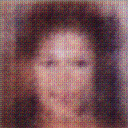
\includegraphics[width=150px]{500_fake_images/samples_5_320.png}%
\caption{A Man In A Suit And Tie Is Smiling}%
\end{figure}

%
\end{document}